


\section{Description of the Solution}
\subsection{Description of the software architecture}



Our software consists of three layers which are Input, Process, and Output layers. Data layer.

\vspace{\baselineskip}

The input layer is responsible for the preprocessing of examination plan files, enabling their utilization within the software.

\vspace{\baselineskip}

The process layer is responsible for analyzing the exam plan data to score, identifying conflicts, and visualizing data based on rules such as ensuring a one-day gap between exams.


\vspace{\baselineskip}

The output data is responsible for representing the scores, conflicts, and charts of every rule in a HTML file.

\FloatBarrier
\begin{figure}[ht]
    \centering
    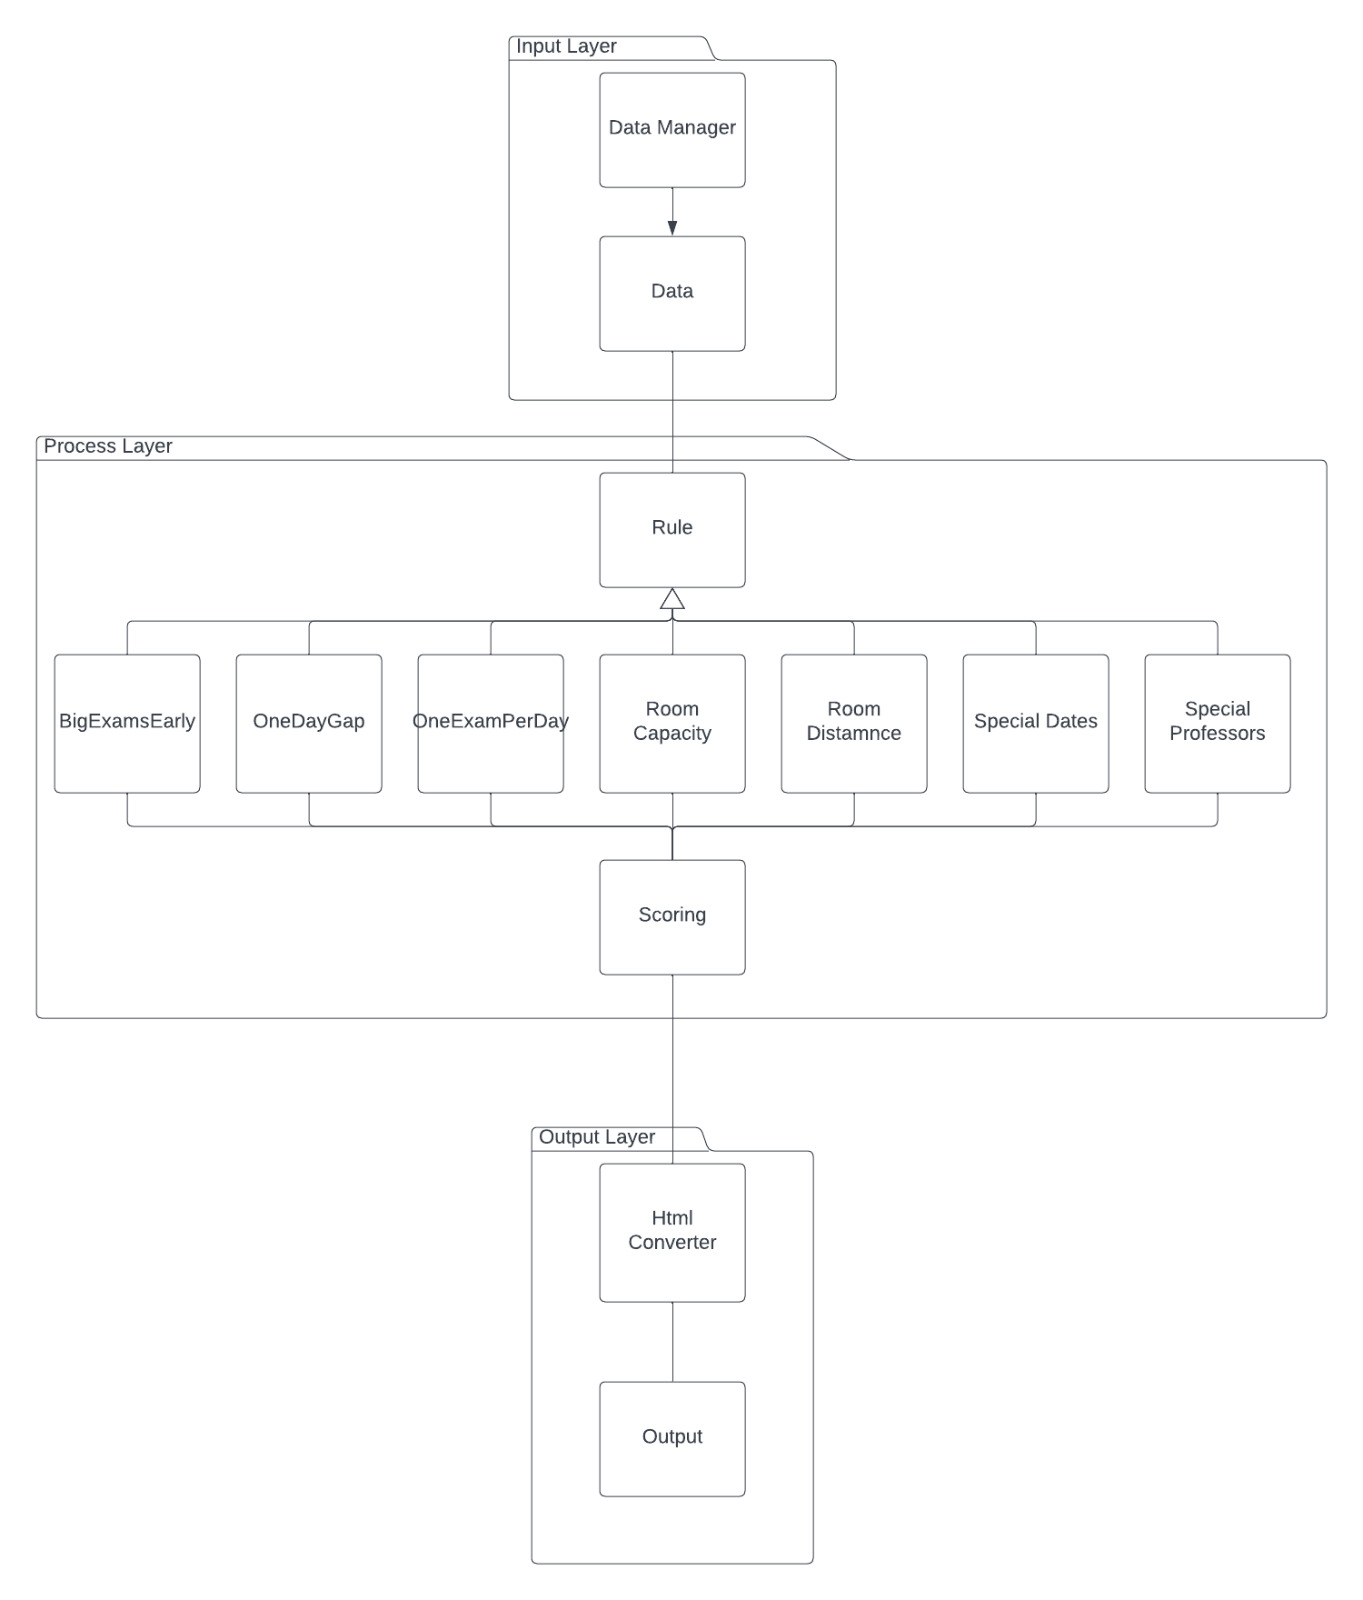
\includegraphics[width=160mm]{images/architecture.jpg}
    \caption{Architecture Design}
    \label{fig:entrance-screen}
\end{figure}
\FloatBarrier



\subsection{Overview and interaction of the components}

\subsubsection{Main Class}


\begin{itemize}
\item This class is responsible from the execution of the program and saving the various html results based on the demand.
\end{itemize}




\subsubsection{Scoring Class}


\begin{itemize}
\item Scoring class interacts with the following rule classes: BigExamsEarly, OneExamPerDay, RoomCapacity, RoomDistance, SpecialProfessors, OneDayGap, SpecialDates.
\item This class is a wrapper for all of the rule classes. It is made to make it easy to access each of the components under one class.
\end{itemize}


\subsubsection{Data Class}


\begin{itemize}
\item The Data class is responsible for importing and organizing the input data from various files.
\item It can load different types of data such as CSV, JSON, and Excel. The following are the files that the Data class interacts with: \texttt{FIW\_Exams\_2022ws.xlsx}, \texttt{Pruefungsanmeldungen\_anonmous.csv}, \texttt{room\_distance\_matrix.xlsx}, \texttt{capacity.json}, \texttt{special\_dates.csv}, \texttt{specific\_professors.xlsx}.
\item It also splits and extracts relevant information from the loaded data and stores them as attributes and methods for further processing.
\item All of the rule classes interact with Data. It is a prerequisite for them to work.
\end{itemize}


\subsubsection{Rule Class}

Rule is the superclass of all scoring classes (such as BigExamsEarly, OneExamPerDay, etc.).

\vspace{\baselineskip}

The class has the following attributes:

\begin{itemize}
\item score.
\item conflicts.
\item plot array.
\end{itemize}
 
It has a method called compute() which returns the score, conflicts, and plot array.

\subsubsection{Data Manager Class}

DataManager is a class to instantiate Data objects. The class provides methods to create and retrieve instances of the Data class. It ensures that only a single instance of the Data class is created and reused throughout the program.

\vspace{\baselineskip}

\subsubsection{BigExamsEarly Class}


\begin{itemize}
\item Big exams should be held early in the exam period, and this class calculates the score and evaluates the exam plan based on the number of big exams and their scheduling time.
\end{itemize}


\subsubsection{OneExamPerDay Class}


\begin{itemize}
\item Verifies whether each student has only one exam scheduled per day.
\item Gives a penalty score while calculating the score of the exam plan based on the number of students who has multiple exams in a day.
\end{itemize}

\subsubsection{OneDayGap Class}


\begin{itemize}
\item This class calculates the score based on the absence of a one-day gap between exams for the same student.
\item basically identifies cases where there is no one-day gap between exams for the same student and calculates a general score for this rule by giving penalty based on the number of conflicts and also draws a plot showing the relationship between the number of conflicts and the score.
\end{itemize}

\subsubsection{RoomCapacity Class}


\begin{itemize}
\item Ensures that the assigned rooms can accommodate the number of students registered for each exam.
\item Computes the score by comparing the number of students with the room capacities for the each exam.
\end{itemize}

\subsubsection{RoomDistance Class}


\begin{itemize}
\item It search the rooms for each exam and if there is more than one room. It calculates the sub-scores of the distance between the relevant rooms.
\item This class has only score as its output.
\end{itemize}

\subsubsection{SpecialDates Class}


\begin{itemize}
\item This class is responsible for calculating the score for examiners, which are not able to come for the exam on a specific day.
\item Checks for conflicts between examiners' names and special dates in the \verb|special_dates_df|.
\item Import data class to reach \verb|special_dates_df| .
\item if there is a match, it adds the conflict information to the 'conflicts' list and makes a binary decision.
\item It returns a percentage score based on whether there is a conflict or not.
\end{itemize}

\subsubsection{SpecialProfessors Class}


\begin{itemize}
\item This class calculates special professors score based on the number of exams and the distance between those exam days that same professors supervise.

\end{itemize}






\subsubsection{Output Class}


\begin{itemize}
\item Handles the generation and saving of output files.
\item Provides methods for saving the results as HTML files. These methods offers two different option either you can get a single result of one rule class or a summary list that includes all results.
\item Utilizes the HtmlConverter class to convert data into HTML format and print the output.
\end{itemize}


\subsubsection{HtmlConverter Class}


\begin{itemize}
\item Converts the processed data into HTML format for output representation.
\item Provides methods for creating HTML pages, and printing the HTML output.

\end{itemize}




 \subsection{Quality Assurance}
 
 \subsubsection{Introduction}

 This document presents the Quality Assurance strategy that has been employed for the evaluation
of our existing examination scheduling system. We utilized Python's unittest framework to
construct and perform unit tests for each rule class in the system.


\vspace{\baselineskip}

Each rule class is thoroughly tested under both the best-case and worst-case scenarios. These
scenarios are represented using a combination of mock data, created within the Test methods for
each test case, and artificial data derived from external files. The objective is to mimic a variety of
real-world scenarios.


\vspace{\baselineskip}

These test cases are organized within a dedicated Test class, containing distinct test methods for
each case. For instance, the test methods \texttt{'test\_big\_exams\_early\_best'},  and  \\ 
\texttt{'test\_big\_exams\_early\_worst'} correspond to the best and worst scenarios of the 'big exams early'
rule respectively.



\vspace{\baselineskip}

Our goal with Quality Assurance is to thoroughly test the exam schedule evaluation system under
different scenarios. This helps to make sure our system is strong, trustworthy, and can accurately
check the quality of any exam schedule. We aim to highlight both what's working well and what
could be better in the schedule.

\subsubsection{Module: OneExamPerDay}

 
\vspace{\baselineskip}

 
\textbf{Test1: One Exam Per Day - Best Scenario}


\vspace{\baselineskip}

 
 \textbf{Test Description:}
This tests uses a dataset where students take a maximum of one exam
per day. It tests the rule under optimal conditions and expects a high score.

\vspace{\baselineskip}

\textbf{Input:}
 Mock data where all students in exam plan take maximum one exam per day.


\vspace{\baselineskip}

\textbf{Expected Result:}
Score is approximately 100 out of 100. This indicates that the scheduling
system is functioning properly for the best-case scenario.



\vspace{\baselineskip}


 
\textbf{Test2: One Exam Per Day - Worst Scenario}


\vspace{\baselineskip}

 
 \textbf{Test Description:}
This tests uses a dataset where students take more than one exam per
day. It tests the rule under optimal conditions and expects a low score.

\vspace{\baselineskip}

\textbf{Input:}
Mock data where all students in exam plan take more than one exam per day.


\vspace{\baselineskip}

 
 \textbf{Expected Result:}
Score is approximately 0 out of 100. This indicates that the scheduling
system is functioning properly for the worst-case scenario.


\vspace{\baselineskip}

\subsubsection{Module: SpecialDates}

 
\vspace{\baselineskip}

 
\textbf{Test1: Special Dates - Best scenario}


\vspace{\baselineskip}

 
 \textbf{Test Description:}
This test uses a dataset where examiners don’t have to supervise exams
in his/her special specific dates.


\vspace{\baselineskip}

\textbf{Input:}
Mock data where all examiners don’t supervise exams in specific dates.



\vspace{\baselineskip}

\textbf{Expected Result:}
Score is approximately 100 out of 100. This indicates that the scheduling
system is functioning properly for the best-case scenario.


\vspace{\baselineskip}


 
\textbf{Test2: Special Dates - Worst scenario}


\vspace{\baselineskip}

 
 \textbf{Test Description:}
 This test uses a dataset where examiners have to supervise exams in
his/her special specific dates.


\vspace{\baselineskip}

\textbf{Input:}
Mock data where all examiners supervise exams in specific dates.


\vspace{\baselineskip}

 
 \textbf{Expected Result:}
 Score is approximately 0 out of 100. This indicates that the scheduling
system is functioning properly for the worst-case scenario.


\vspace{\baselineskip}



 \subsubsection{Module: BigExamsEarly}

 
\vspace{\baselineskip}

 
 \textbf{Test 1: Big Exams Early - Best Scenario}


\vspace{\baselineskip}

 
 \textbf{Test Description:}
 This test uses a dataset where the bigger exams are scheduled early. It tests
the rule under optimal conditions and expects a high score.


\vspace{\baselineskip}


 \textbf{Input:}
 Mock data where larger exams are scheduled earlier in the exam schedule.


\vspace{\baselineskip}

 
 \textbf{Expected Result:}
 Score is greater or equal to 70. This indicates that the scheduling system is
functioning properly for the best-case scenario and bigger exams are indeed scheduled earlier.


\vspace{\baselineskip}

 
 \textbf{Test 2: Big Exams Early - Worst Scenario}


\vspace{\baselineskip}

 
 \textbf{Test Description:}
This test uses a dataset where the bigger exams are scheduled late. It tests the
rule under the worst conditions and expects a low score.


\vspace{\baselineskip}


 \textbf{Input:}
 Mock data where larger exams are scheduled later in the exam schedule.


\vspace{\baselineskip}

 
 \textbf{Expected Result:}
 Score is less or equal to 5. This indicates that the scheduling system properly
penalizes scenarios where bigger exams occur late in the schedule.


\vspace{\baselineskip}



 \subsubsection{Module: RoomDistance}

 
\vspace{\baselineskip}


 
 \textbf{Test 1: Room Distance - Best Scenario}


\vspace{\baselineskip}

 
 \textbf{Test Description:}
 This test uses a dataset where students are allocated in rooms close to each
other. It tests the rule under optimal conditions and expects a high score.


\vspace{\baselineskip}


 \textbf{Input:}
A combination of mock data that is either directly created as a dataframe or drawn from
artificial datasets like Excel files. Both types of data are later assigned to the attributes of the
Mock class. This dataset simulates a situation where students' allocated exam rooms are in close
proximity, thus representing an optimal scenario for the room distance rule.

\vspace{\baselineskip}

 
 \textbf{Expected Result:}
 Score is approximately equal to 100. This indicates that the scheduling system
is functioning properly for the best-case scenario and the exams are scheduled in rooms close to
each other.


\vspace{\baselineskip}

 
 \textbf{Test 2: Room Distance - Worst Scenario}


\vspace{\baselineskip}

 
 \textbf{Test Description:}
This test uses a dataset where students are allocated in rooms far from each
other. It tests the rule under the worst conditions and expects a low score.


\vspace{\baselineskip}


 \textbf{Input:}
 A combination of mock data that is either directly created as a dataframe or drawn from
artificial datasets like Excel files. Both types of data are later assigned to the attributes of the
Mock class. This dataset simulates a situation where students' allocated exam rooms are far
apart, thus representing the worst-case scenario for the room distance rule.


\vspace{\baselineskip}

 
 \textbf{Expected Result:}
Score is approximately equal to 0. This indicates that the scheduling system
properly penalizes scenarios where exams are scheduled in rooms far from each other.


\vspace{\baselineskip}



 \subsubsection{Module: OneDayGap}

 
\vspace{\baselineskip}


 
 \textbf{Test 1: One Day Gap - Best Scenario}


\vspace{\baselineskip}

 
 \textbf{Test Description:}
 This test uses a dataset where students have at least one day gap between
their exams. It tests the rule under optimal conditions and expects a score close to 100, indicating
no conflicts.
\vspace{\baselineskip}


 \textbf{Input:}
Mock data (coming from artificial datasets like Excel files, which are passed to the Data
class as parameters), where all students have at least one day gap between their exams.

\vspace{\baselineskip}

 
 \textbf{Expected Result:}
Score is approximately equal to 0, indicating there are no back-to-back exams
for students, which is the ideal scenario.


\vspace{\baselineskip}

 
 \textbf{Test 2: One Day Gap - Worst Scenario}


\vspace{\baselineskip}

 
 \textbf{Test Description:}
This test uses a dataset where students do not have a one day gap between
their exams. It tests the rule under the worst conditions and expects a score close to 0, indicating
high conflicts.

\vspace{\baselineskip}


 \textbf{Input:}
 Mock data where students have exams without a day gap.
 
\vspace{\baselineskip}

 
 \textbf{Expected Result:}
Score is approximately equal to 0. The score is expected to be low, indicating
that the system correctly identifies the situation where students have exams without a one day
gap as a problematic scheduling scenario.


\vspace{\baselineskip}




 \subsubsection{Module: SpecialProfessors}

 
\vspace{\baselineskip}


 
 \textbf{Test 1: Special Professors - Best Scenario}


\vspace{\baselineskip}

 
 \textbf{Test Description:}
This test uses a dataset where special professors have all their exams
scheduled on the same day. It tests the rule under optimal conditions and expects a score close
to 100, indicating no conflicts.

\vspace{\baselineskip}


 \textbf{Input:}
Mock data where all special professors are assigned to multiple examinations on the same
day (for each professor individually), rather than having their exams spread out over separate
days.

\vspace{\baselineskip}

 
 \textbf{Expected Result:}
Score is approximately equal to 100, indicating that all special professors'
exams are scheduled on the same day. This means they aren't required to come to campus on
multiple, separate days, which is the ideal scenario.


\vspace{\baselineskip}

 
 \textbf{Test 2: Special Professors - Worst Scenario}


\vspace{\baselineskip}

 
 \textbf{Test Description:}
This test uses a dataset where special professors are assigned to supervise
examinations on different days, implying they have to be present on campus on multiple separate
days. This is considered the worst-case scenario for this rule and expects a score close to 0,
indicating a large number of conflicts.

\vspace{\baselineskip}


 \textbf{Input:}
Mock data where special professors are assigned to supervise different examinations, each
on a separate day. This is achieved by intentionally designing the mock data such that each
special professor supervises one examination per day, but the exams are scheduled on different
days.
 
\vspace{\baselineskip}

 
 \textbf{Expected Result:}
Score is approximately equal to 0, indicating that special professors' exams are
distributed over several days. This is the least ideal scenario, as it means these special professors
have to come to campus on multiple, separate days, creating a high level of inconvenience.

\vspace{\baselineskip}




 \subsubsection{Module: RoomCapacity}

 
\vspace{\baselineskip}


 
 \textbf{Test 1: Room Capacity - Best Scenario}


\vspace{\baselineskip}

 
 \textbf{Test Description:}
This test uses mock data where the number of students and the capacity of
exam rooms are nearly identical. It tests the room capacity rule under optimal conditions and
expects a high score, indicating the rooms' capacity is efficiently utilized.

\vspace{\baselineskip}


 \textbf{Input:}
Mock data, directly created within the test function, representing a scenario where the
number of students in each course nearly matches the capacity of the assigned exam rooms.

\vspace{\baselineskip}

 
 \textbf{Expected Result:}
Score is greater than or equal to 80, which indicates that room capacities are
efficiently used and there is a balance between the number of students and room capacities. This
implies a proper utilization of resources and an optimal exam scheduling.

\vspace{\baselineskip}

 
 \textbf{Test 2: Room Capacity - Worst Scenario}


\vspace{\baselineskip}

 
 \textbf{Test Description:}
This test uses mock data where the number of students is significantly lower
than the capacity of the assigned exam rooms. It tests the room capacity rule under worst-case
conditions and expects a low score, indicating inefficient usage of room capacities.

\vspace{\baselineskip}


 \textbf{Input:}
Mock data, directly created within the test function, representing a scenario where the
number of students for each course is significantly lower than the capacity of the assigned exam
rooms.
 
\vspace{\baselineskip}

 
 \textbf{Expected Result:}
Score is less than or equal to 10, indicating that the room capacities are not
efficiently used and there is a significant imbalance between the number of students and room
capacities. This implies an inefficient utilization of resources and sub-optimal exam scheduling.

\vspace{\baselineskip}

\subsubsection{Test Results Interpretation}


If all the tests pass, it indicates that the scoring system for the module is working as
expected under both the best and worst scenarios.

\vspace{\baselineskip}


• If any of the tests fail, it suggests a problem with the scoring system in handling that specific
scenario. The console output and failure messages should provide insight into what went
wrong in these cases. The problem may stem from how the score is calculated or how the
input data is processed.